%==================================
%          Introduction
%==================================
\section{\review{Introduction}}


%----------------------------------
%           Motivation
%----------------------------------
%\subsection{\review{Motivation}}

Beam-based measurements have been carried in the LHC since Run 1 to better understand the decapolar
fields. Those have been carried out via chromaticity
measurements~\cite{maclean_non-linear_2011,maclean_commissioning_2016,maclean_measurement_2014}. 
The third order of the non-linear chromaticity, $Q'''$, which is expected to be generated for the
most part by decapolar errors in the main dipoles, has shown a consistent discrepancy at injection
energy between its expected value from simulations and that observed.
\Cref{fig:decapoles:bare_chroma_vs_simulations} illustrates this discrepancy, highlighting a factor
$-2$ between the supposedly corrected machine and the corrected model.

\begin{figure}[!htb]
    \centering
    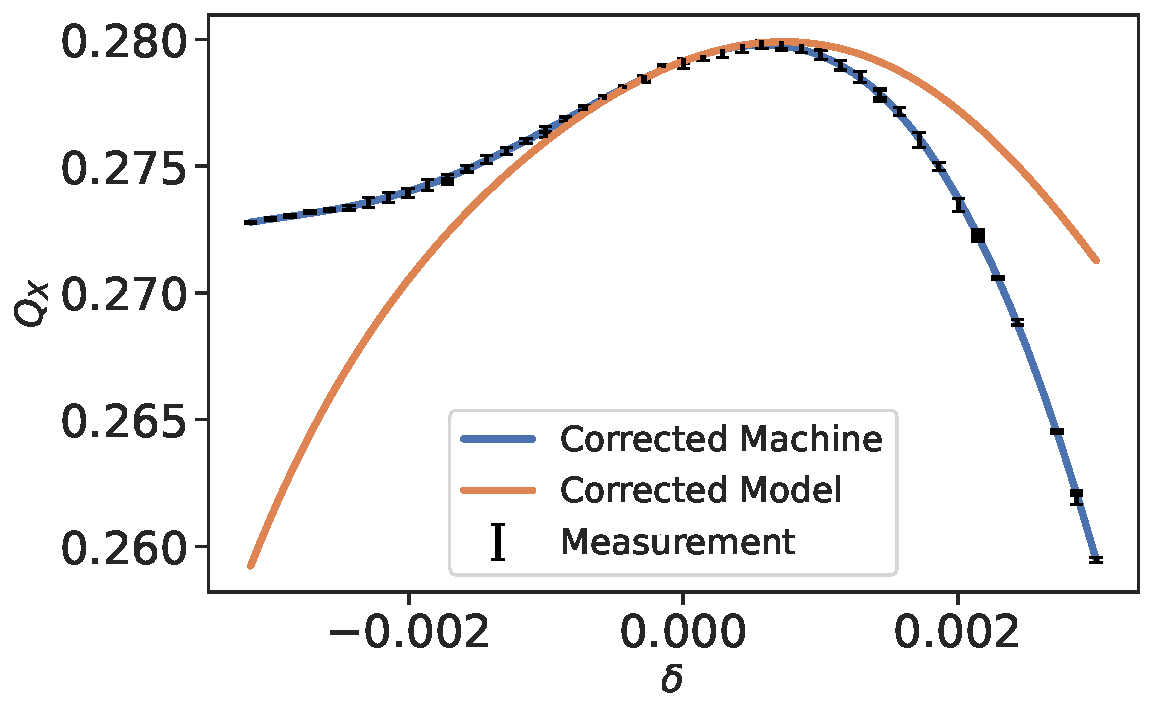
\includegraphics[width=0.8\textwidth]{images/dq3_corrected_simulation_fidel.pdf}
    \caption{Measured and simulated chromaticity with application of the nominal decapolar
    corrections from FiDeL. It can be seen that although the corrections should diminish $Q'''$, it
    is not well corrected in practice.}
    \label{fig:decapoles:bare_chroma_vs_simulations}
\end{figure}

The FiDeL model, based on magnetic measurements, is used during operation to correct various
multipole errors in the LHC, including octupolar and decapolar. The operational corrections being
based on this magnetic model and simulations, the residual $Q'''$ value is expected to be small,
which is however not the case.  Chromaticity measurements have thus been repeated during LHC's Run 3
and corrections made routine, aimed at correcting the observed discrepancy.

While the study of non-linear chromaticity has proven valuable in identifying the existence of this
discrepancy, it does not yet permit alone to understand its exact origins. In an effort to gain
deeper insights, additional measurements were performed focusing on novel observables that had not
been previously explored.
\textit{Bare chromaticity} involves measuring chromaticity with
the octupolar an decapolar correctors deactivated ; this approach aims to isolate the machine
effects from those of the correctors.
\textit{Chromatic amplitude detuning}, evaluates how the tune varies with both the beam's action and
the momentum offset ; this methods has the benefit of having a different expression from that of the
chromaticity, to rule out exclusively momentum dependent effects, such a higher-order dispersion.

In addition to previous measurements, direct measurements of decapolar Resonance Driving Terms
(RDTs) were conducted for the first time in the LHC, at injection energy. These high-order RDTs,
which influence resonances near the working point, have also benefited from corrections, marking the
first instance of directly correcting such high-order terms, using a response matrix-based approach.
During the study of these resonances, lower-order multipoles, such as sextupoles and octupoles, were
found to be significant contributors. Their effects are thoroughly derived and examined, as they are
expected to strongly impact the dynamic aperture at injection energy.

While lower-order field errors in the LHC are generally well understood and controlled, this is not
the case for higher-order errors such as decapoles and beyond. Precise control of these higher-order
non-linearities is expected to be crucial for future colliders like the FCC, where decapolar field
corrections will play a large role in maintaining an optimal dynamic aperture. Extending advanced
beam-based measurement and correction techniques to higher-order errors is therefore of significant
interest.
The observed discrepancy in the correction of third-order chromaticity ($Q'''$) points to an
incomplete understanding of both the error sources and the magnetic model. Addressing this gap is
essential for improving higher-order corrections in the LHC and preparing for the challenges of the
next generation of accelerators.
